\section{Performance}

L'implementazione di un modello ad albero per la parallelizzazione di eventi
di proliferazione cellulare si è rivelata una tecnica efficiente per questo
tipo di problema, di seguito in figura ritroviamo i risultati ottenuti per
quanto riguarda i tempi necessari alla computazione della simulazione
modificando il parametro $\tau_{max}$.
\\
\begin{figure}[H]
    \begin{minipage}[b]{.5\linewidth}
        \centering
        \scalebox{0.6}{
        \begin{tikzpicture}
            \begin{axis}[legend style={at={(0.95,0.4)}},
                    xtick=data,
                    ymode=log,
                    log ticks with fixed point,
                    xlabel={$\tau_{max}$},
                    ylabel={simulation time (s)}
                ]
                \addplot table {Data/Comparison/fit_python.txt};
                \addplot table {Data/Comparison/fit_tesla_k80.txt};
                \legend{Python,Tesla K80}
            \end{axis}
        \end{tikzpicture}
        }
        \subcaption{Fitting $\varphi_{min}=11.0, \tau_{max}=240$}
    \end{minipage}
    \begin{minipage}[b]{.5\linewidth}
        \centering
        \scalebox{0.6}{
        \begin{tikzpicture}
            \begin{axis}[legend style={at={(0.95,0.4)}},
                    xtick=data,
                    ymode=log,
                    log ticks with fixed point,
                    xlabel={$\tau_{max}$},
                    ylabel={simulation time (s)}
                ]
                \addplot table {Data/Comparison/validation_python.txt};
                \addplot table {Data/Comparison/validation_gtx_970.txt};
                \legend{Python,GTX 970}
            \end{axis}
        \end{tikzpicture}
        }
        \subcaption{Validation $\varphi_{min}=8.7, \tau_{max}=504$}
    \end{minipage}
    \caption{}
\end{figure}

Un'idea ancora più generale riguardo allo speedup guadagnato è fornita dal
seguente grafico
\\
\begin{figure}[H]
    \begin{minipage}[b]{.5\linewidth}
        \centering
        \scalebox{0.6}{
        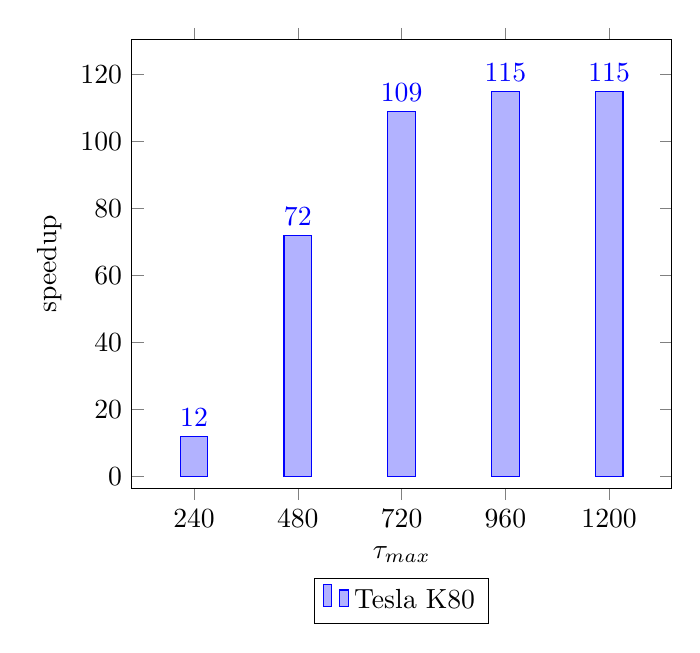
\begin{tikzpicture}
            \begin{axis}[
                ybar,
                enlargelimits=0.15,
                legend style={at={(0.5,-0.20)},
                anchor=north,legend columns=-1},
                ylabel={speedup},
                xlabel={$\tau_{max}$},
                symbolic x coords={240,480,720, 960, 1200},
                xtick=data,
                nodes near coords,
                nodes near coords align={vertical},
            ]
            \addplot coordinates {
                (240, 12) (480, 72) (720, 109) (960, 115) (1200, 115)
            };
            \legend{Tesla K80}
            \end{axis}
        \end{tikzpicture}
        }
        \subcaption{Fitting $\varphi_{min}=11.0, \tau_{max}=240$}
    \end{minipage}
    \begin{minipage}[b]{.5\linewidth}
        \centering
        \scalebox{0.6}{
        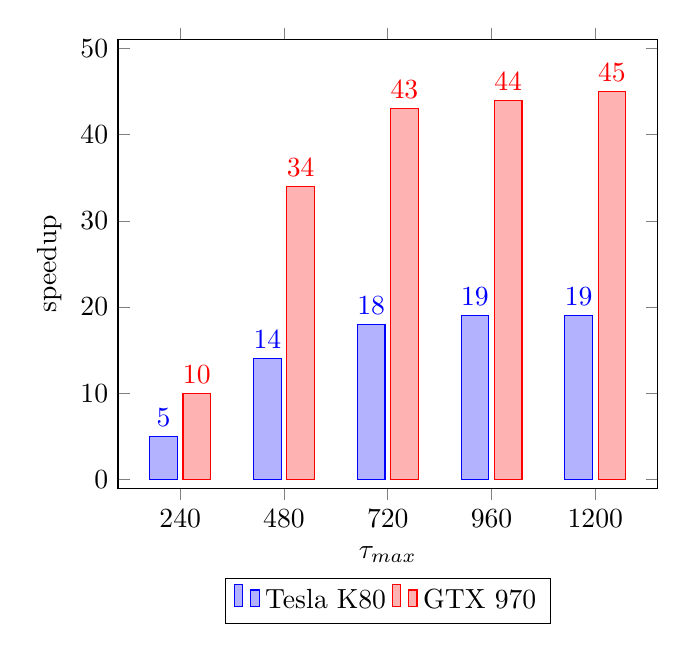
\begin{tikzpicture}
            \begin{axis}[
                ybar,
                enlargelimits=0.15,
                legend style={at={(0.5,-0.20)},
                anchor=north,legend columns=-1},
                ylabel={speedup},
                xlabel={$\tau_{max}$},
                symbolic x coords={240,480,720, 960, 1200},
                xtick=data,
                nodes near coords,
                nodes near coords align={vertical},
            ]
            \addplot coordinates {
                (240, 5) (480, 14) (720, 18) (960, 19) (1200, 19)
            };
            \addplot coordinates {
                (240, 10) (480, 34) (720, 43) (960, 44) (1200, 45)
            };
            \legend{Tesla K80, GTX 970}
            \end{axis}
        \end{tikzpicture}
        }
        \subcaption{Validation $\varphi_{min}=8.7, \tau_{max}=504$}
    \end{minipage}
    \caption{}
\end{figure}

Come è possibile notare per quanto riguarda la \textit{validazione}, la scheda
GTX 970 è più performante della Tesla K80. Questo è dato dal fatto che
la GTX 970 possiede un clock di 1050 MHz, mentre la Tesla K80 solamente di
562 MHz, dunque frequenza quasi dimezzata. Questo impatta leggermente sulle
performance a causa della ricerca binaria implementata nel calcolo
dell'istogramma finale, dato che un thread deve eseguire un loop per la ricerca
della fluorescenza $\varphi_{i}$ all'interno dell'array delle frequenze $\Omega$.
Sebbene la ricerca binaria sia nell'ordine di $O(\log_{2}{n})$, con un clock
minore si rischia di avere un leggero calo di performance rispetto a schede
con clock maggiori.
